\documentclass[final,5p,times,twocolumn]{elsarticle}

\usepackage{amssymb}
\usepackage{amsmath}
\usepackage{mathtools}
\usepackage{booktabs}
\usepackage{multirow}
\usepackage{graphicx}
\usepackage{url}
\usepackage{enumitem}
\usepackage{microtype}

\journal{Computers \& Operations Research}

\begin{document}

\begin{frontmatter}

\title{Dynamic ICU Bed Allocation Under Resource Scarcity: A Discrete-Event Simulation Integrating Multi-Type Beds and Triage Policies}

\author[ufma]{Carlos Eduardo Veras Gomes}
\ead{carlos.evg@discente.ufma.br}

\author[ufma]{Jo\~ao Augusto Ferreira Nunes de Carvalho}
\ead{augusto.joa@discente.ufma.br}

\author[ufma]{Francisco Glaubos Nunes Cl\'imaco\corref{cor1}}
\ead{francisco.glaubos@ufma.br}

\cortext[cor1]{Corresponding author}

\affiliation[ufma]{organization={Federal University of Maranh\~ao (UFMA)},
            addressline={Av. dos Portugueses, 1966, Bacanga},
            city={S\~ao Lu\'is},
            postcode={65080-805},
            state={MA},
            country={Brazil}}

\begin{abstract}
During epidemic surges and mass-casualty events, intensive care bed capacity is often exceeded and hospitals must triage continuous stochastic arrivals across specialized units. Static one-shot formulations miss waiting-time deterioration, severity-dependent length of stay (LOS), and bed coupling. We develop a discrete-event simulation of a tertiary Brazilian university hospital with four CNES-calibrated intensive-care pools (adult, coronary, pediatric, neonatal; 55 beds) and bidirectional adult--coronary overflow. Survival probabilities deteriorate exponentially while patients wait; LOS increases with severity, creating an explicit trade-off between marginal benefit and bed-days consumed. Six policies are compared under Common Random Numbers: First-Come, First-Served (FCFS), Most/Least Serious First (MSF/LSF), Marginal Gain for Survival (MGS), a $c\mu$-style index (CMU-MGS), and a deadline-aware austere rule (AUSTERE). Only bed capacities are empirical; clinical distributions are synthetic and are stress-tested under observation noise. Over a 15-day warm-up and 60-day evaluation window ($100$ replications; Holm--Bonferroni adjustment), occupancy reaches $99.9\%$ under severe surge ($\rho=1.6$). Relative to FCFS, CMU-MGS and MGS preserve $+58.57$ [$57.45$, $59.70$] and $+57.79$ [$56.71$, $58.88$] expected lives ($+11.3\%$ and $+11.2\%$; both $p_{\mathrm{Holm}}<10^{-300}$). Gains remain material under noisy $\widetilde{\Delta P}$ ($\sigma\le 0.2$). The contribution is not that greedy $\Delta P$ beats weak heuristics in a tautological model, but that benefit-per-bed-day ranking remains dominant once deterioration, severity--LOS coupling, overflow, and imperfect information are present.
\end{abstract}

\begin{highlights}
\item DES of multi-type ICU triage with deterioration and severity-dependent LOS.
\item HU-UFMA/CNES capacities (55 beds) with adult--coronary overflow coupling.
\item Six policies compared under CRN, including $c\mu$ and austere deadline rules.
\item At $\rho{=}1.6$, CMU-MGS saves $+58.6$ expected lives vs FCFS ($11.3\%$).
\item Ranking is robust to noisy $\widetilde{\Delta P}$ estimates ($\sigma$ up to $0.2$).
\end{highlights}

\begin{keyword}
Healthcare operations research \sep Intensive care units \sep Discrete-event simulation \sep Triage policies \sep Bed allocation \sep Queueing with abandonment
\end{keyword}

\end{frontmatter}

\section{Introduction}
\label{sec:intro}

Intensive Care Units (ICUs) are among the most constrained resources in acute care. When demand surges---as during COVID-19 waves or mass-casualty disasters---hospitals must decide which critically ill patients receive scarce beds and which are managed in lower-acuity settings \cite{grasselli2020critical, aquino2022ethical, craxi2020rationing, dieteren2022should}. Chronologic First-Come, First-Served (FCFS) queues are operationally simple but ignore prognosis and therapeutic benefit \cite{White_2021, Frej_2021}.

A substantial operations research literature already studies ICU admission control \cite{kim2015association}, discharge timing \cite{chan2012optimizing}, mass-casualty prioritization \cite{mills2013resource}, and triage under austere conditions with deterioration \cite{sun2018patient}. Parallel work develops static portfolio or multi-criteria ICU allocation models \cite{Frej_2021, Frej_2023, White_2021}. What remains comparatively under-studied for multi-specialty referral hospitals is the joint effect of (i)~continuous multi-pool dynamics, (ii)~clinical deterioration while waiting, (iii)~severity-dependent bed holding times, and (iv)~strong OR benchmarks such as benefit-per-bed-day indices and deadline-aware rules.

Real tertiary ICUs are not a single pooled server farm:
\begin{enumerate}[label=(\roman*)]
    \item Arrivals and discharges are asynchronous; triage is re-solved whenever a bed frees \cite{Bilbao_2022, Valeva_2023}.
    \item Neonatal, pediatric and adult beds are clinically non-fungible, while adult medical ICU and coronary care may share limited overflow flexibility \cite{king2019modelling}.
    \item Prolonged queueing induces deterioration and reneging before ICU salvage is possible \cite{Murray_2023, sun2018patient}.
\end{enumerate}

This paper develops a discrete-event simulation (DES) for that setting and makes three contributions:
\begin{itemize}
    \item \textbf{Non-tautological dynamic triage model.} Survival probability conditional on ICU admission decays with waiting time; expected LOS increases with severity. Marginal benefit and bed consumption are therefore in tension, so greedy $\Delta P$ is no longer an automatic maximizer of expected survivors.
    \item \textbf{Hospital-calibrated multi-pool structure with coupling.} Capacities are taken from CNES records for HU-UFMA (55 intensive beds across neonatal, pediatric, adult and coronary pools), with bidirectional adult--coronary overflow. Pediatric and neonatal pools remain segregated.
    \item \textbf{Stronger benchmarks and statistical reporting.} We compare FCFS, MSF, LSF, Marginal Gain for Survival (MGS), a $c\mu$-style index CMU-MGS, and an austere deadline-aware rule AUSTERE inspired by \cite{sun2018patient}, under Common Random Numbers (CRN), paired confidence intervals, relative effects and Holm--Bonferroni adjustment, plus sensitivity to noisy $\widetilde{\Delta P}$.
\end{itemize}

Section~\ref{sec:works} reviews related work. Section~\ref{sec:modeling} formalizes the model. Section~\ref{sec:experiments} documents parameters and experimental design. Section~\ref{sec:results} reports results. Section~\ref{sec:limitations} discusses limitations. Section~\ref{sec:conclusion} concludes.

\section{Related Work}
\label{sec:works}

Table~\ref{tab:lit_comparison} situates the present study relative to representative ICU and crisis-triage models.

\begin{table*}[t]
\centering
\caption{Comparison with selected ICU allocation and crisis-triage literature.}
\label{tab:lit_comparison}
\resizebox{\textwidth}{!}{%
\begin{tabular}{lcccccc}
\toprule
\textbf{Study} & \textbf{Horizon} & \textbf{Bed structure} & \textbf{Arrivals / LOS} & \textbf{Deterioration} & \textbf{Abandonment} & \textbf{Triage focus} \\
\midrule
Kim et al.\ \cite{kim2015association} & Dynamic & Adult ICU & Empirical & Indirect & Diversion & Admission control \\
Chan et al.\ \cite{chan2012optimizing} & Dynamic & Adult ICU & Empirical & Readmission & --- & Discharge timing \\
Mills et al.\ \cite{mills2013resource} & Dynamic & Mass-casualty & Fluid / sim. & Time-dependent survival & --- & Resource-based priority \\
Sun et al.\ \cite{sun2018patient} & Dynamic & Austere triage & Stochastic & Explicit & Deadlines & Index / austere policies \\
Argon \& Ziya \cite{argon2009priority} & Queueing & Classes & Markovian & --- & --- & Imperfect type info \\
Alban et al.\ \cite{Alban_2020} & Dynamic & Adult COVID ICU & Process sim. & --- & Overflow & Capacity thresholds \\
Frej et al.\ \cite{Frej_2021,Frej_2023} & Static & Single pool & Batch & --- & No & Utility / Bayesian \\
White \& Lo \cite{White_2021} & Static & Single pool & --- & --- & No & Multi-principle ethics \\
Valeva et al.\ \cite{Valeva_2023} & Dynamic & ICU + step-down & Markovian & --- & Blocking & Acuity outflow \\
Bilbao \cite{Bilbao_2022} & Dynamic & Adult ICU & Non-hom.\ Poisson / phase-type & --- & Yes & Admission / early discharge \\
\textbf{This work} & \textbf{DES} & \textbf{4 pools + overflow} & \textbf{Poisson / log-normal} & \textbf{Yes} & \textbf{Yes} & \textbf{MGS, $c\mu$, austere, MSF/LSF, FCFS} \\
\bottomrule
\end{tabular}}
\end{table*}

Kim et al.\ \cite{kim2015association} link ICU congestion to admission decisions and outcomes. Chan et al.\ \cite{chan2012optimizing} optimize discharge under readmission risk. Mills et al.\ \cite{mills2013resource} and Sun et al.\ \cite{sun2018patient} show that prioritization should internalize resource use and deteriorating survival under austere conditions; Argon and Ziya \cite{argon2009priority} study prioritization under imperfect type information. Static multi-criteria ICU models \cite{Frej_2021, Frej_2023, White_2021} formalize ethics and uncertainty but abstract away continuous queue dynamics. Capacity and step-down simulations \cite{Alban_2020, Bilbao_2022, Valeva_2023} emphasize adult systems. Our contribution is a hospital-calibrated multi-type DES that embeds deterioration, severity--LOS coupling, adult--coronary overflow and imperfect $\Delta P$ information against stronger OR benchmarks.

\section{Dynamic Simulation Model}
\label{sec:modeling}

\subsection{System state and events}

Consider a tertiary hospital over horizon $[0,T]$. Intensive-care pools are
\[
J=\{\text{neonatal},\text{pediatric},\text{adult},\text{coronary}\},
\]
with capacities $C_j$ and total $C=\sum_j C_j$. Pediatric and neonatal beds are exclusive. Adult and coronary beds admit bidirectional overflow: an adult patient may occupy a free coronary bed, and conversely, when the home queue is empty.

Patients arrive as independent Poisson processes with rates $\lambda_j$. Patient $i$ has attributes
\begin{equation}
\bigl(j(i),\, t_{\mathrm{arr}}^i,\, P_{\mathrm{out}}^i,\, P_{\mathrm{in},0}^i,\, \mathrm{LOS}_i,\, \mathbb{E}[\mathrm{LOS}_i],\, W_{\max}^i,\, u_i\bigr).
\end{equation}
Here $P_{\mathrm{out}}^i$ is ward/no-ICU survival; $P_{\mathrm{in},0}^i$ is immediate-admission ICU survival; $W_{\max}^i$ is the reneging tolerance; and $u_i\sim\mathrm{Unif}(0,1)$ is an independent outcome draw, generated from a dedicated random stream separate from arrivals, clinical covariates and LOS.

Clinical deterioration while waiting is modeled by exponential decay of the salvageable margin:
\begin{equation}
P_{\mathrm{in}}^i(t)=P_{\mathrm{out}}^i+\bigl(P_{\mathrm{in},0}^i-P_{\mathrm{out}}^i\bigr)\,e^{-\alpha(t-t_{\mathrm{arr}}^i)},
\label{eq:det}
\end{equation}
so the instantaneous marginal gain is $\Delta P_i(t)=P_{\mathrm{in}}^i(t)-P_{\mathrm{out}}^i$. Severity-dependent LOS creates bed-time tension:
\begin{equation}
\mathbb{E}[\mathrm{LOS}_i]=\mu_{\mathrm{los}}\bigl(0.6+\beta(1-P_{\mathrm{out}}^i)\bigr),\qquad
\mathrm{LOS}_i\sim\mathrm{LogNormal}(\cdot),
\label{eq:los}
\end{equation}
with coefficient of variation $CV_{\mathrm{los}}$. Thus high-severity patients tend to consume more bed-days.

The event engine processes arrivals, discharges and timeouts. If patient $i$ reaches $t_{\mathrm{arr}}^i+W_{\max}^i$ without admission, the patient reneges and receives survival probability $P_{\mathrm{out}}^i$. Bed cleaning time and early discharge transfers are not modeled; discharge frees the bed at $t_{\mathrm{adm}}^i+\mathrm{LOS}_i$.

Each replication uses a warm-up of $T_w$ days and an evaluation window $[T_w,T]$. Metrics are computed only for patients with $t_{\mathrm{arr}}^i\in[T_w,T)$. Patients still queued at $T$ contribute $P_{\mathrm{out}}^i$ to expected survival if not admitted; bed-time after $T$ does not enter the occupancy integral. Occupancy of pool $j$ is the time-average
\begin{equation}
\bar{\mathcal{O}}_j=\frac{1}{(T-T_w)C_j}\int_{T_w}^{T} B_j(t)\,dt,
\end{equation}
and global occupancy aggregates bed-time over all pools.

\subsection{Triage policies}
\label{sec:policies}

When a bed in pool $j$ frees at time $t$ and eligible candidates exist (home queue, or adult/coronary overflow), policy $\pi$ selects
\begin{equation}
i^*=\arg\max_{i\in\mathcal{Q}_j^{\mathrm{elig}}(t)} s_i^{\pi}(t),
\end{equation}
with earlier arrival as tie-break. Scores are:
\begin{align}
s_i^{\mathrm{FCFS}}(t) &= -t_{\mathrm{arr}}^i,\\
s_i^{\mathrm{MSF}}(t) &= 1-P_{\mathrm{out}}^i,\\
s_i^{\mathrm{LSF}}(t) &= P_{\mathrm{in}}^i(t),\\
s_i^{\mathrm{MGS}}(t) &= \Delta P_i(t),\\
s_i^{\mathrm{CMU\text{-}MGS}}(t) &= \frac{\Delta P_i(t)}{\mathbb{E}[\mathrm{LOS}_i]},\\
s_i^{\mathrm{AUSTERE}}(t) &= \frac{\Delta P_i(t)}{\mathbb{E}[\mathrm{LOS}_i]}\left(1+\frac{1}{\tau_i(t)}\right),
\end{align}
where $\tau_i(t)=\max\{0.05,\, t_{\mathrm{arr}}^i+W_{\max}^i-t\}$ is residual time to reneging. MGS denotes \emph{Marginal Gain for Survival} (not ``maximizing overall survival expectation'' as a claim of optimality). MSF ranks physiological urgency via low $P_{\mathrm{out}}$; it is not claimed to implement the ethical ``rule of rescue,'' because it ignores salvageability. CMU-MGS is a $c\mu$-style benefit-per-bed-day index \cite{smith1956various}. AUSTERE adds deadline urgency in the spirit of austere triage with deterioration \cite{sun2018patient}. Under imperfect information, decision makers observe $\widetilde{\Delta P}_i(t)=\mathrm{clip}_{[0,1]}(\Delta P_i(t)+\varepsilon_i)$ with $\varepsilon_i\sim\mathcal{N}(0,\sigma^2)$ \cite{argon2009priority}.

\subsection{Performance metrics}

Let $\mathcal{A}^{\pi}$ be patients arriving in the evaluation window and admitted under $\pi$. Expected survivors are
\begin{equation}
S_{\mathrm{exp}}^{\pi}=\sum_{i\in\mathcal{A}^{\pi}} P_{\mathrm{in}}^i(t_{\mathrm{adm}}^i)+\sum_{i\notin\mathcal{A}^{\pi}} P_{\mathrm{out}}^i.
\label{eq:sexp}
\end{equation}
Realized survivors replace probabilities by indicators $\mathbb{I}(u_i<\cdot)$ using the dedicated outcome stream. We report admissions, reneging rate, mean wait of admitted patients, mean wait of reneged patients, pool-specific occupancy/admissions, and paired differences $\Delta S_r^{\pi}=S_{\mathrm{exp},r}^{\pi}-S_{\mathrm{exp},r}^{\mathrm{FCFS}}$.

\section{Experimental Design}
\label{sec:experiments}

\subsection{What is and is not calibrated}

Capacities are taken from DATASUS/CNES (competency 12/2024; establishment 2111302726653) for HU-UFMA \cite{cnes_datasus_huufma}: $C_{\mathrm{neonatal}}=20$, $C_{\mathrm{pediatric}}=10$, $C_{\mathrm{adult}}=15$, $C_{\mathrm{coronary}}=10$ ($C=55$). Public HU-UFMA spreadsheets on admissions and ward LOS do not provide ICU-specific $P_{\mathrm{in}}/P_{\mathrm{out}}$, severity-stratified LOS, or reneging tolerances \cite{dados_abertos_huufma,bittencourt2006sistema,machado2016qualidade}. Accordingly, clinical distributions below are synthetic and identical across pools unless noted; we do not claim empirical clinical calibration. Arrival rates are set by a common demand ratio $\rho$ via Little's law,
\begin{equation}
\lambda_j=\frac{\rho\, C_j}{\mu_{\mathrm{los}}},
\end{equation}
so all pools face the same nominal congestion level $\rho\in\{0.7,1.0,1.3,1.6\}$.

\subsection{Synthetic clinical parameters and protocol}

Unless stated otherwise: $\mu_{\mathrm{los}}=5$~days, $CV_{\mathrm{los}}=0.6$, $\beta=0.8$, $\alpha=0.10$~day$^{-1}$,
$P_{\mathrm{out}}\sim\mathrm{Unif}(0.05,0.65)$,
$P_{\mathrm{in},0}=P_{\mathrm{out}}+(1-P_{\mathrm{out}})g$ with $g\sim\mathrm{Unif}(0.10,0.80)$,
and $W_{\max}\sim\mathrm{Unif}(1,3)$~days. Warm-up $T_w=15$~days; horizon $T=75$~days (60-day evaluation). Each $(\rho,\pi)$ pair uses $100$ CRN-synchronized replications ($2{,}400$ trajectories). Paired tests against FCFS are adjusted by Holm--Bonferroni over all $20$ comparisons. Software: Python~3.12; seeds are stream-specific SHA-256 digests of $(\mathrm{seed},\rho,\mathrm{replication},\mathrm{stream})$. Code and processed outputs accompany the repository.

\section{Results}
\label{sec:results}

\subsection{Occupancy integrity and overall performance}

Table~\ref{tab:dynamic_results} summarizes policy performance. Under $\rho=0.7$, global occupancy is about $77\%$--$78\%$ and reneging is rare ($\approx 1.4\%$--$1.9\%$). Under $\rho=1.6$, occupancy reaches $99.8\%$--$99.9\%$ while roughly $42\%$--$47\%$ of arrivals renege: beds are essentially saturated whenever queues persist, consistent with Little's law after warm-up and severity-inflated LOS (implied mean LOS $\approx 5.6$~days from bed-days/admissions).

\begin{table*}[t]
\centering
\caption{Mean performance over the 60-day evaluation window ($100$ replications). Waiting times are reported separately for admitted and reneged patients.}
\label{tab:dynamic_results}
\resizebox{\textwidth}{!}{%
\begin{tabular}{clcccccc}
\toprule
$\rho$ & Policy & Admitted & Reneging (\%) & Wait$_{\mathrm{adm}}$ (h) & Wait$_{\mathrm{ren}}$ (h) & Occupancy (\%) & Exp.\ survivors \\
\midrule
\multirow{6}{*}{0.7}
 & FCFS & 457.0 & 1.4 & 2.8 & 33.0 & 77.7 & 294.2 \\
 & MSF & 454.5 & 1.9 & 2.0 & 39.8 & 77.3 & 294.5 \\
 & LSF & 454.8 & 1.8 & 1.9 & 39.5 & 77.2 & 294.4 \\
 & AUSTERE & 456.9 & 1.4 & 2.7 & 40.7 & 77.6 & 295.0 \\
 & MGS & 454.6 & 1.9 & 1.9 & 40.5 & 77.3 & 294.9 \\
 & CMU-MGS & 454.6 & 1.9 & 1.9 & 40.6 & 77.3 & 294.9 \\
\midrule
\multirow{6}{*}{1.0}
 & FCFS & 571.7 & 13.4 & 16.9 & 35.6 & 96.6 & 387.8 \\
 & MSF & 558.0 & 15.5 & 9.3 & 43.5 & 95.8 & 395.2 \\
 & LSF & 569.4 & 13.8 & 8.5 & 43.6 & 95.2 & 396.6 \\
 & AUSTERE & 571.1 & 13.5 & 15.3 & 46.8 & 96.6 & 398.5 \\
 & MGS & 562.1 & 14.9 & 8.8 & 44.0 & 95.6 & 401.8 \\
 & CMU-MGS & 563.5 & 14.7 & 8.7 & 44.0 & 95.5 & 401.9 \\
\midrule
\multirow{6}{*}{1.3}
 & FCFS & 585.9 & 31.6 & 30.1 & 37.5 & 99.5 & 450.6 \\
 & MSF & 560.5 & 34.5 & 14.3 & 45.3 & 99.3 & 469.9 \\
 & LSF & 600.2 & 29.9 & 12.9 & 45.2 & 99.1 & 476.1 \\
 & AUSTERE & 582.9 & 31.9 & 26.8 & 47.8 & 99.6 & 474.4 \\
 & MGS & 575.1 & 32.9 & 13.3 & 45.6 & 99.2 & 488.1 \\
 & CMU-MGS & 580.2 & 32.3 & 13.2 & 45.6 & 99.2 & 488.6 \\
\midrule
\multirow{6}{*}{1.6}
 & FCFS & 590.1 & 44.1 & 37.0 & 38.8 & 99.9 & 517.7 \\
 & MSF & 555.8 & 47.3 & 15.8 & 46.1 & 99.9 & 546.7 \\
 & LSF & 616.6 & 41.6 & 14.0 & 46.2 & 99.8 & 556.7 \\
 & AUSTERE & 584.7 & 44.6 & 32.4 & 48.2 & 99.9 & 549.7 \\
 & MGS & 578.2 & 45.2 & 14.3 & 46.3 & 99.8 & 575.4 \\
 & CMU-MGS & 585.1 & 44.5 & 14.2 & 46.3 & 99.8 & 576.2 \\
\bottomrule
\end{tabular}}
\end{table*}

Figure~\ref{fig:survivors} shows expected survivors rising with $\rho$ for all policies, with CMU-MGS and MGS pulling ahead as scarcity intensifies. Absolute survivor counts increase with $\rho$ because more patients arrive; the clinically relevant signal is the gap versus FCFS.

\begin{figure}[ht]
\centering
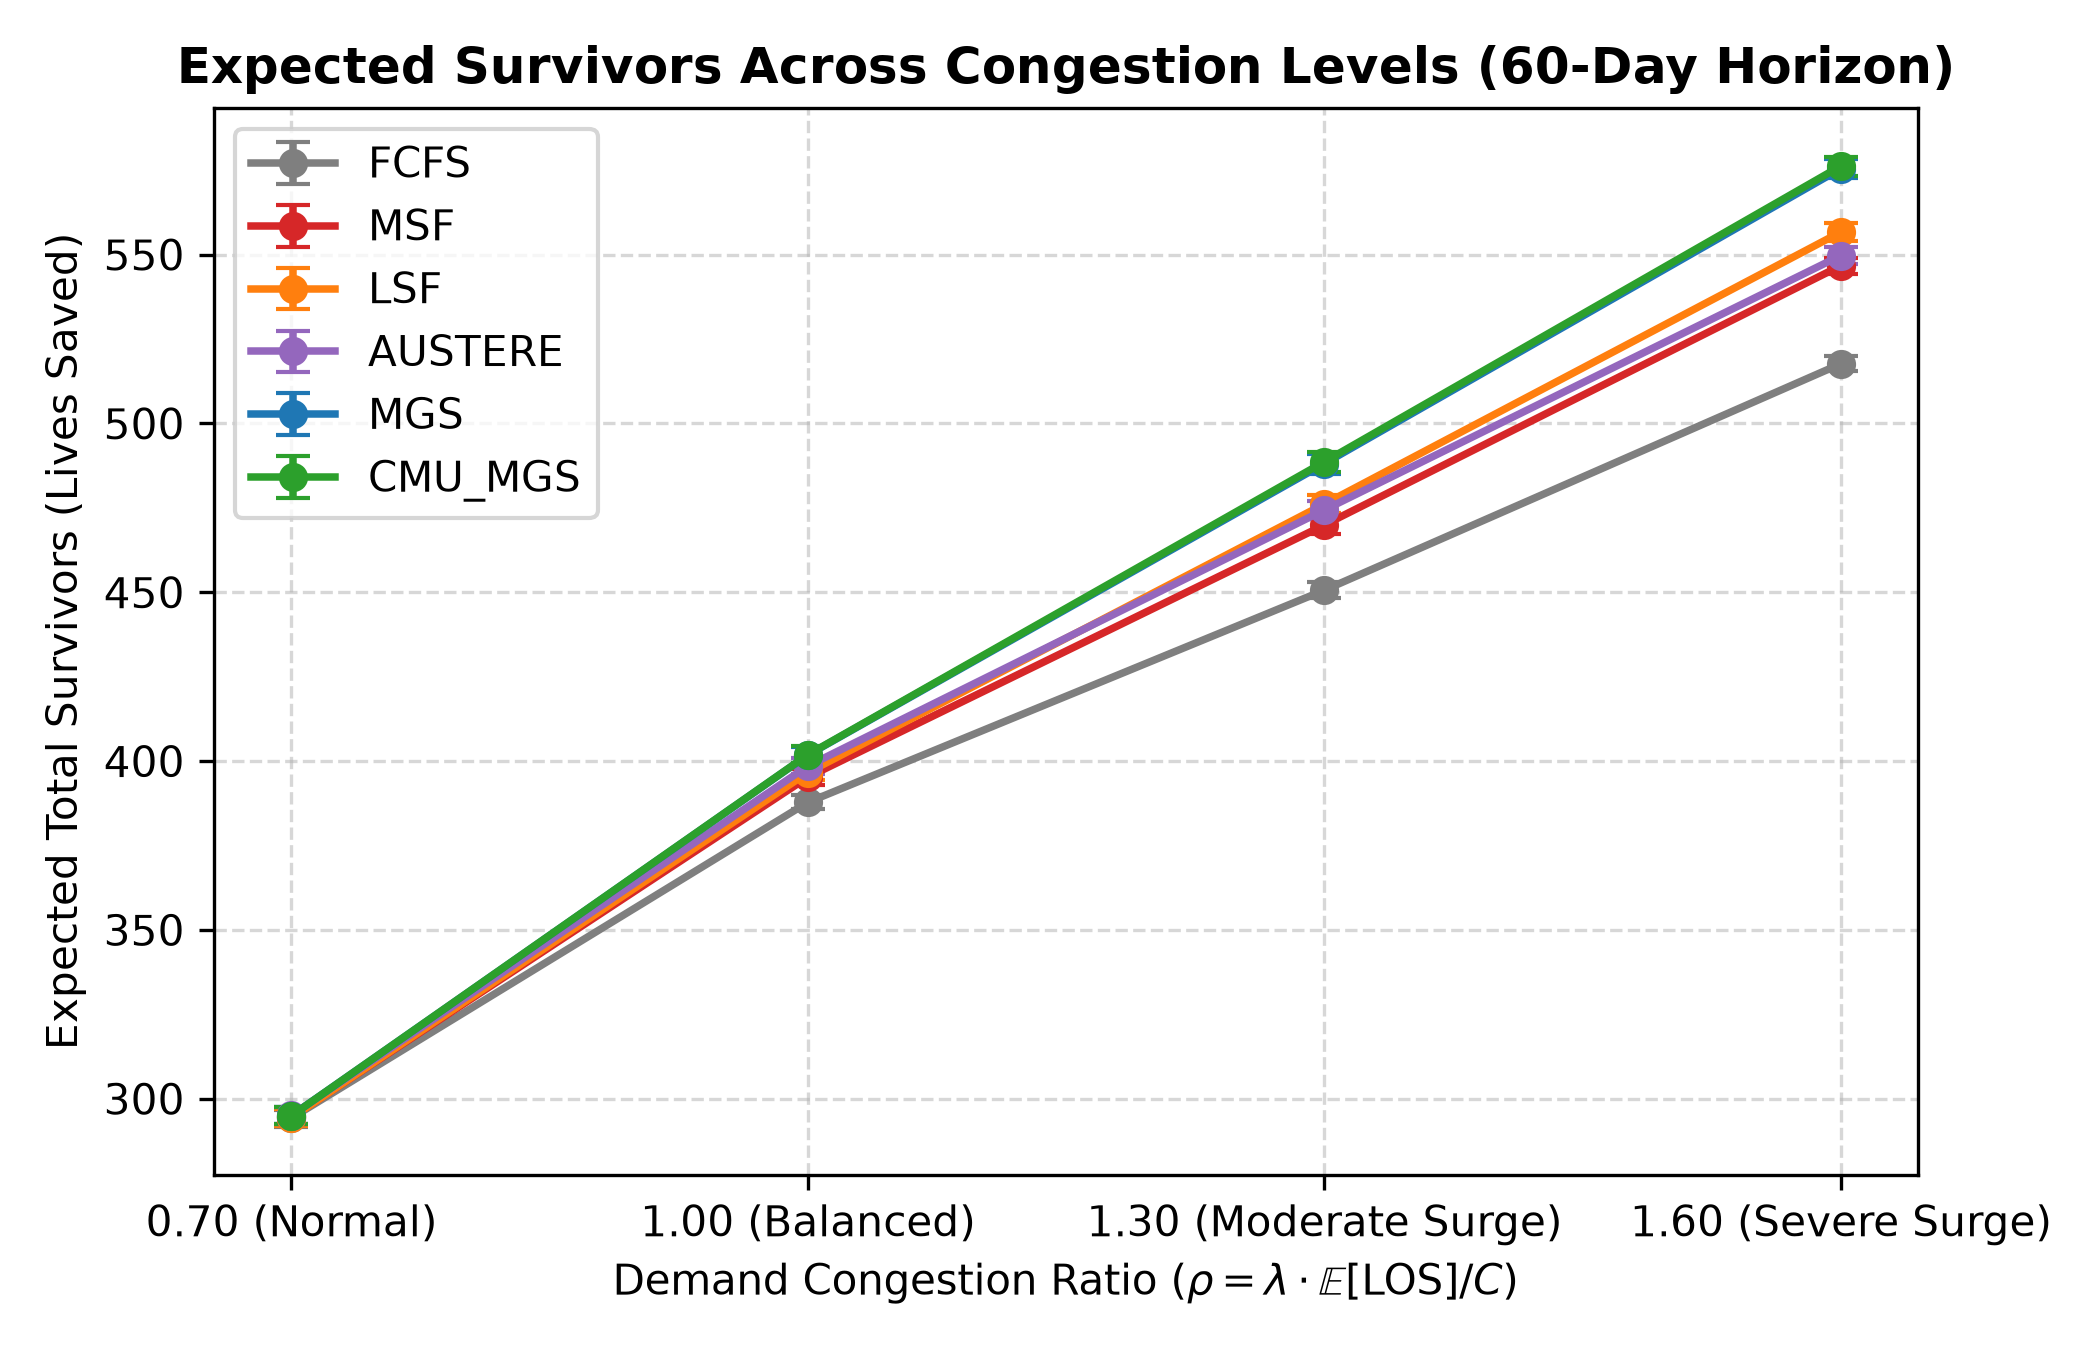
\includegraphics[width=\columnwidth]{fig_survivors.png}
\caption{Expected survivors by policy and demand ratio (evaluation window; error bars are $95\%$ CRN-based intervals).}
\label{fig:survivors}
\end{figure}

\subsection{Paired gains, practical magnitude and multiple testing}

Table~\ref{tab:paired_stats} reports paired differences versus FCFS with $95\%$ intervals, relative effects and Holm-adjusted $p$-values. At $\rho=0.7$, several differences are statistically detectable under CRN (e.g., AUSTERE $+0.80$ [$0.65$, $0.96$]), but relative gains are below $0.3\%$ and operationally negligible. The previous abstract claim of ``statistical indistinguishability at $\rho=0.7$'' was incorrect and is withdrawn. Large $t$-statistics under CRN indicate precise detection of differences, not automatic practical importance; relative percentages and intervals are therefore emphasized.

\begin{table}[ht]
\centering
\caption{Paired expected-survival gain versus FCFS (Holm--Bonferroni over 20 tests).}
\label{tab:paired_stats}
\resizebox{\columnwidth}{!}{%
\begin{tabular}{llcccc}
\toprule
$\rho$ & Policy & $\Delta S$ & $95\%$ CI & Rel.\ \% & $p_{\mathrm{Holm}}$ \\
\midrule
\multirow{5}{*}{0.7}
 & MSF & $+0.23$ & $[0.09,0.36]$ & $+0.08$ & $2.2{\times}10^{-3}$ \\
 & LSF & $+0.14$ & $[-0.01,0.28]$ & $+0.05$ & $0.065$ \\
 & AUSTERE & $+0.80$ & $[0.65,0.96]$ & $+0.27$ & $<10^{-20}$ \\
 & MGS & $+0.71$ & $[0.53,0.88]$ & $+0.24$ & $<10^{-14}$ \\
 & CMU-MGS & $+0.70$ & $[0.52,0.87]$ & $+0.24$ & $<10^{-14}$ \\
\midrule
\multirow{5}{*}{1.0}
 & MSF & $+7.46$ & $[6.91,8.01]$ & $+1.92$ & $<10^{-150}$ \\
 & LSF & $+8.84$ & $[8.29,9.39]$ & $+2.28$ & $<10^{-200}$ \\
 & AUSTERE & $+10.75$ & $[10.14,11.35]$ & $+2.77$ & $<10^{-260}$ \\
 & MGS & $+14.02$ & $[13.27,14.76]$ & $+3.61$ & $<10^{-290}$ \\
 & CMU-MGS & $+14.09$ & $[13.34,14.85]$ & $+3.63$ & $<10^{-280}$ \\
\midrule
\multirow{5}{*}{1.3}
 & MSF & $+19.31$ & $[18.62,19.99]$ & $+4.28$ & $<10^{-300}$ \\
 & LSF & $+25.51$ & $[24.65,26.37]$ & $+5.66$ & $<10^{-300}$ \\
 & AUSTERE & $+23.75$ & $[22.94,24.56]$ & $+5.27$ & $<10^{-300}$ \\
 & MGS & $+37.48$ & $[36.47,38.50]$ & $+8.32$ & $<10^{-300}$ \\
 & CMU-MGS & $+38.02$ & $[37.00,39.04]$ & $+8.44$ & $<10^{-300}$ \\
\midrule
\multirow{5}{*}{1.6}
 & MSF & $+29.06$ & $[28.07,30.06]$ & $+5.61$ & $<10^{-300}$ \\
 & LSF & $+39.03$ & $[38.02,40.04]$ & $+7.54$ & $<10^{-300}$ \\
 & AUSTERE & $+32.07$ & $[31.03,33.11]$ & $+6.20$ & $<10^{-300}$ \\
 & MGS & $+57.79$ & $[56.71,58.88]$ & $+11.16$ & $<10^{-300}$ \\
 & CMU-MGS & $+58.57$ & $[57.45,59.70]$ & $+11.32$ & $<10^{-300}$ \\
\bottomrule
\end{tabular}}
\end{table}

\begin{figure}[ht]
\centering
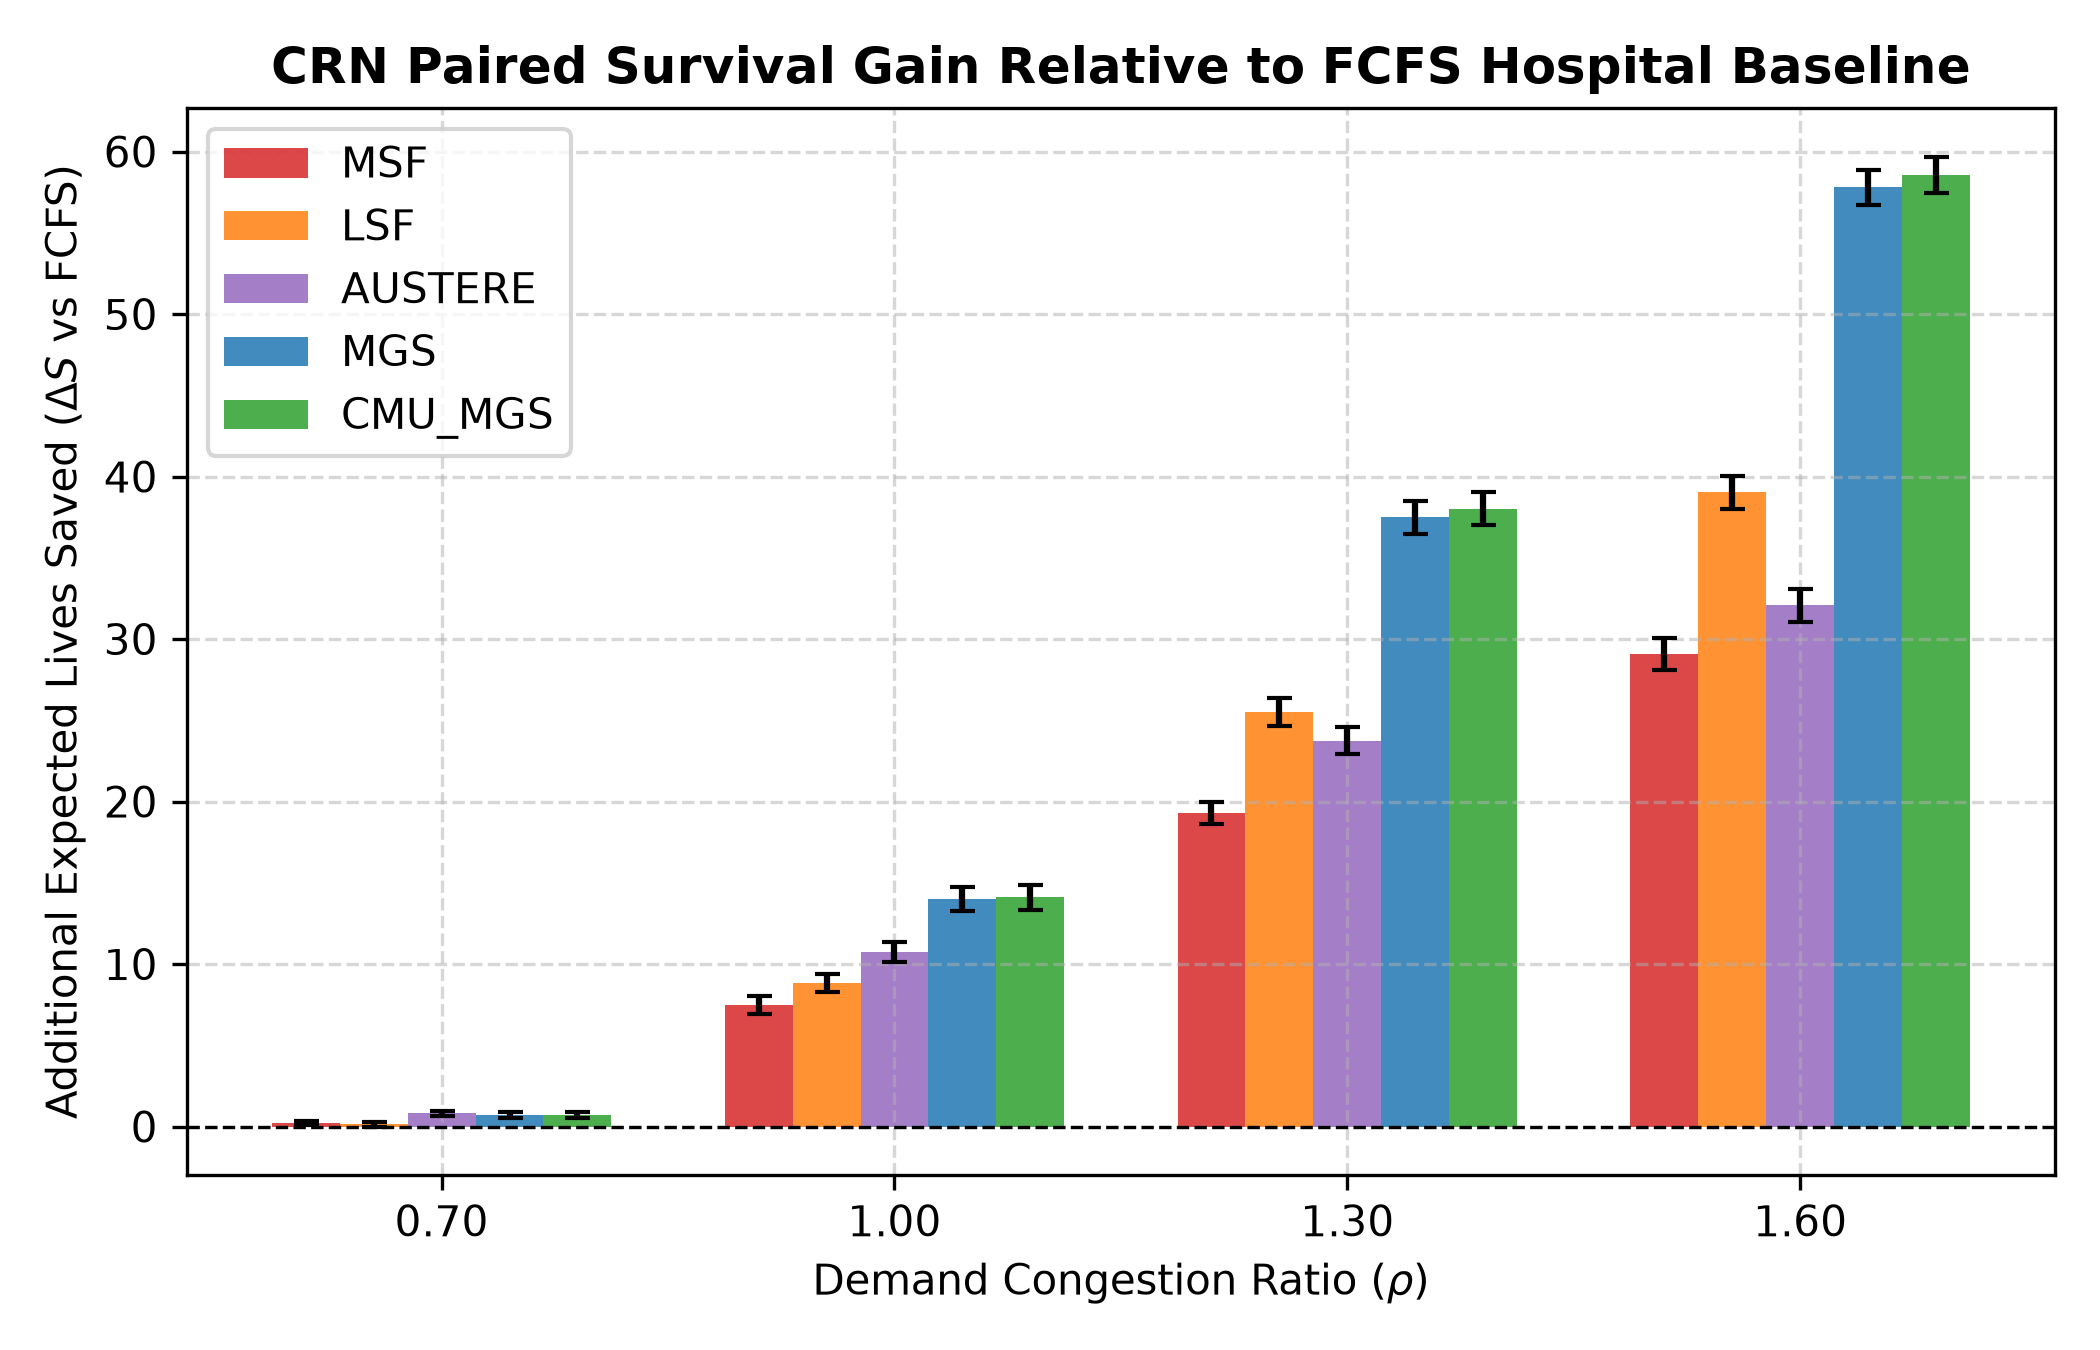
\includegraphics[width=\columnwidth]{fig_paired_gain.png}
\caption{Paired additional expected lives versus FCFS ($95\%$ intervals). CMU-MGS and MGS dominate as congestion rises.}
\label{fig:paired_gain}
\end{figure}

At $\rho=1.6$, CMU-MGS and MGS dominate all benchmarks, including AUSTERE and LSF (Figure~\ref{fig:paired_gain}). The $c\mu$-style index slightly edges pure MGS ($576.2$ vs $575.4$ expected survivors), consistent with the severity--LOS trade-off in Eqs.~\eqref{eq:det}--\eqref{eq:los}.

\subsection{Waiting times, reneging and per-pool outcomes}

Figure~\ref{fig:waiting_times} separates admitted-patient waits from reneging rates. Priority rules do not ``release beds faster'': LOS is exogenous to the policy. Shorter admitted waits under MGS/CMU-MGS/LSF arise because new high-priority arrivals jump the queue while low-priority patients more often hit $W_{\max}$. FCFS admitted waits reach $37.0$~h at $\rho=1.6$, versus $14.2$--$14.3$~h under CMU-MGS/MGS; reneging remains high for all policies once capacity is saturated.

\begin{figure*}[t]
\centering
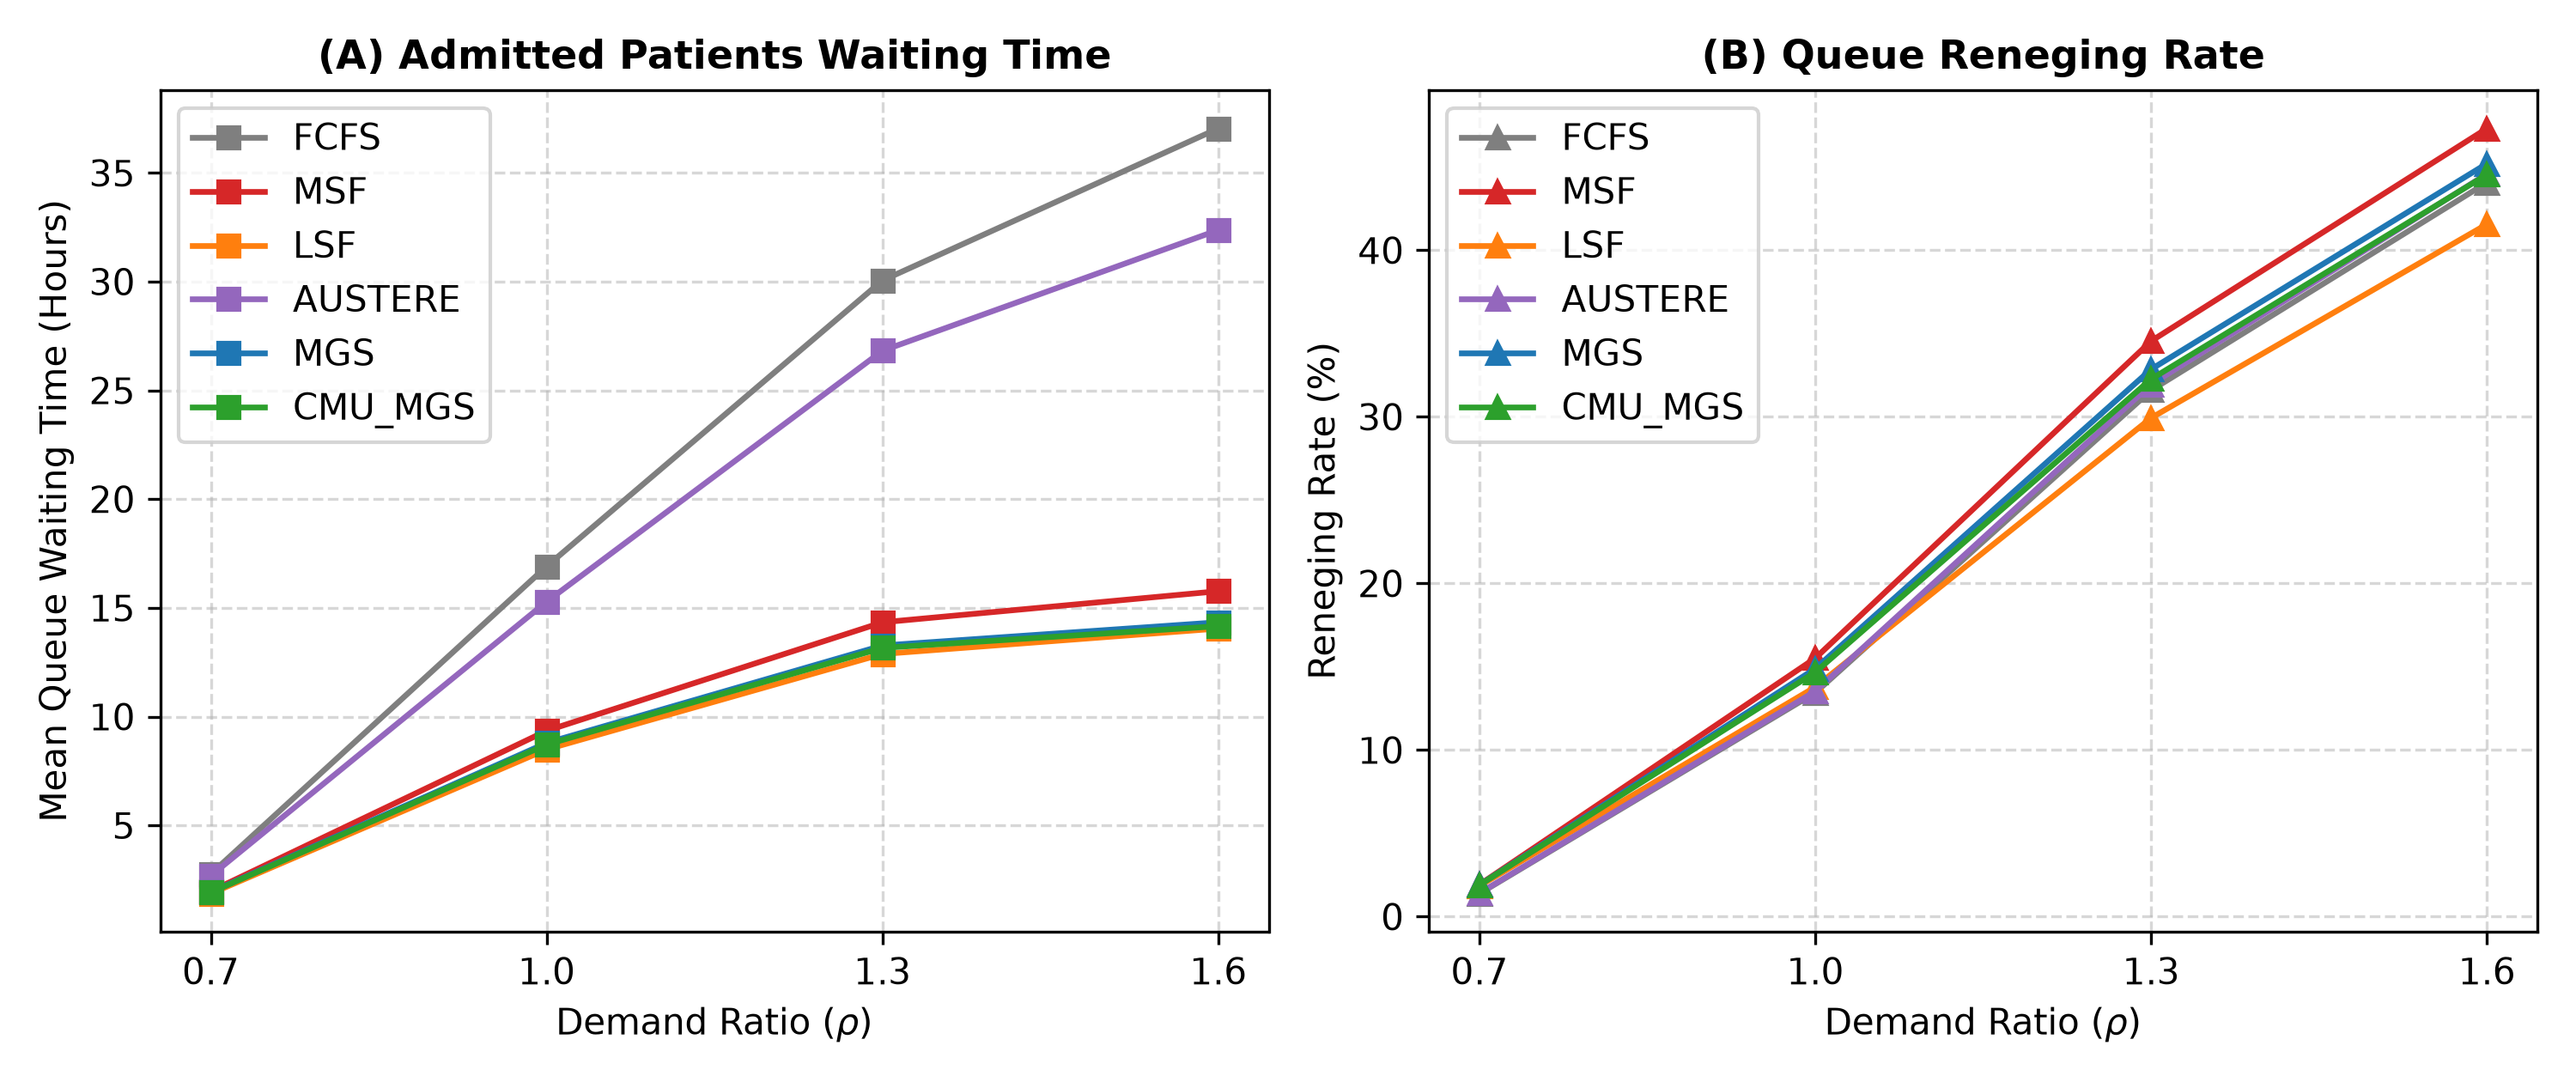
\includegraphics[width=\textwidth]{fig_waiting_times.png}
\caption{(A)~Mean waiting time of admitted patients; (B)~reneging rate. Priority disciplines cut admitted waits but do not eliminate crisis-level reneging.}
\label{fig:waiting_times}
\end{figure*}

Table~\ref{tab:pool} reports pool-level admissions and occupancy at $\rho=1.6$. Adult and coronary pools are essentially full under all policies; overflow couples them without merging pediatric/neonatal capacity. Neonatal volume dominates absolute admissions because of its larger capacity.

\begin{table}[ht]
\centering
\caption{Mean admissions and occupancy by pool at $\rho=1.6$.}
\label{tab:pool}
\resizebox{\columnwidth}{!}{%
\begin{tabular}{llcccc}
\toprule
Policy & Metric & Adult & Coronary & Pediatric & Neonatal \\
\midrule
\multirow{2}{*}{FCFS}
 & Admitted & 162.7 & 105.5 & 106.9 & 215.1 \\
 & Occupancy (\%) & 100.0 & 100.0 & 99.7 & 100.0 \\
\multirow{2}{*}{MGS}
 & Admitted & 160.6 & 104.0 & 104.9 & 208.7 \\
 & Occupancy (\%) & 100.0 & 100.0 & 99.3 & 99.9 \\
\multirow{2}{*}{CMU-MGS}
 & Admitted & 162.3 & 104.7 & 106.5 & 211.5 \\
 & Occupancy (\%) & 100.0 & 100.0 & 99.3 & 99.9 \\
\multirow{2}{*}{AUSTERE}
 & Admitted & 161.8 & 104.1 & 106.3 & 212.5 \\
 & Occupancy (\%) & 100.0 & 100.0 & 99.6 & 100.0 \\
\bottomrule
\end{tabular}}
\end{table}

\subsection{Robustness to noisy marginal-benefit estimates}

Figure~\ref{fig:sensitivity} evaluates FCFS, AUSTERE, MGS and CMU-MGS at $\rho=1.6$ when decisions use noisy $\widetilde{\Delta P}$ ($\sigma\in\{0,0.05,0.10,0.20\}$; $50$ replications). FCFS is unaffected. MGS/CMU-MGS degrade gracefully: at $\sigma=0.20$ they still preserve about $+39$ expected lives over FCFS ($553.8$/$553.1$ vs $515.0$), remaining ahead of AUSTERE ($543.5$). Exact $\Delta P$ knowledge is therefore not required for material gains, though equity impacts of mis-ranking deserve clinical scrutiny.

\begin{figure}[ht]
\centering
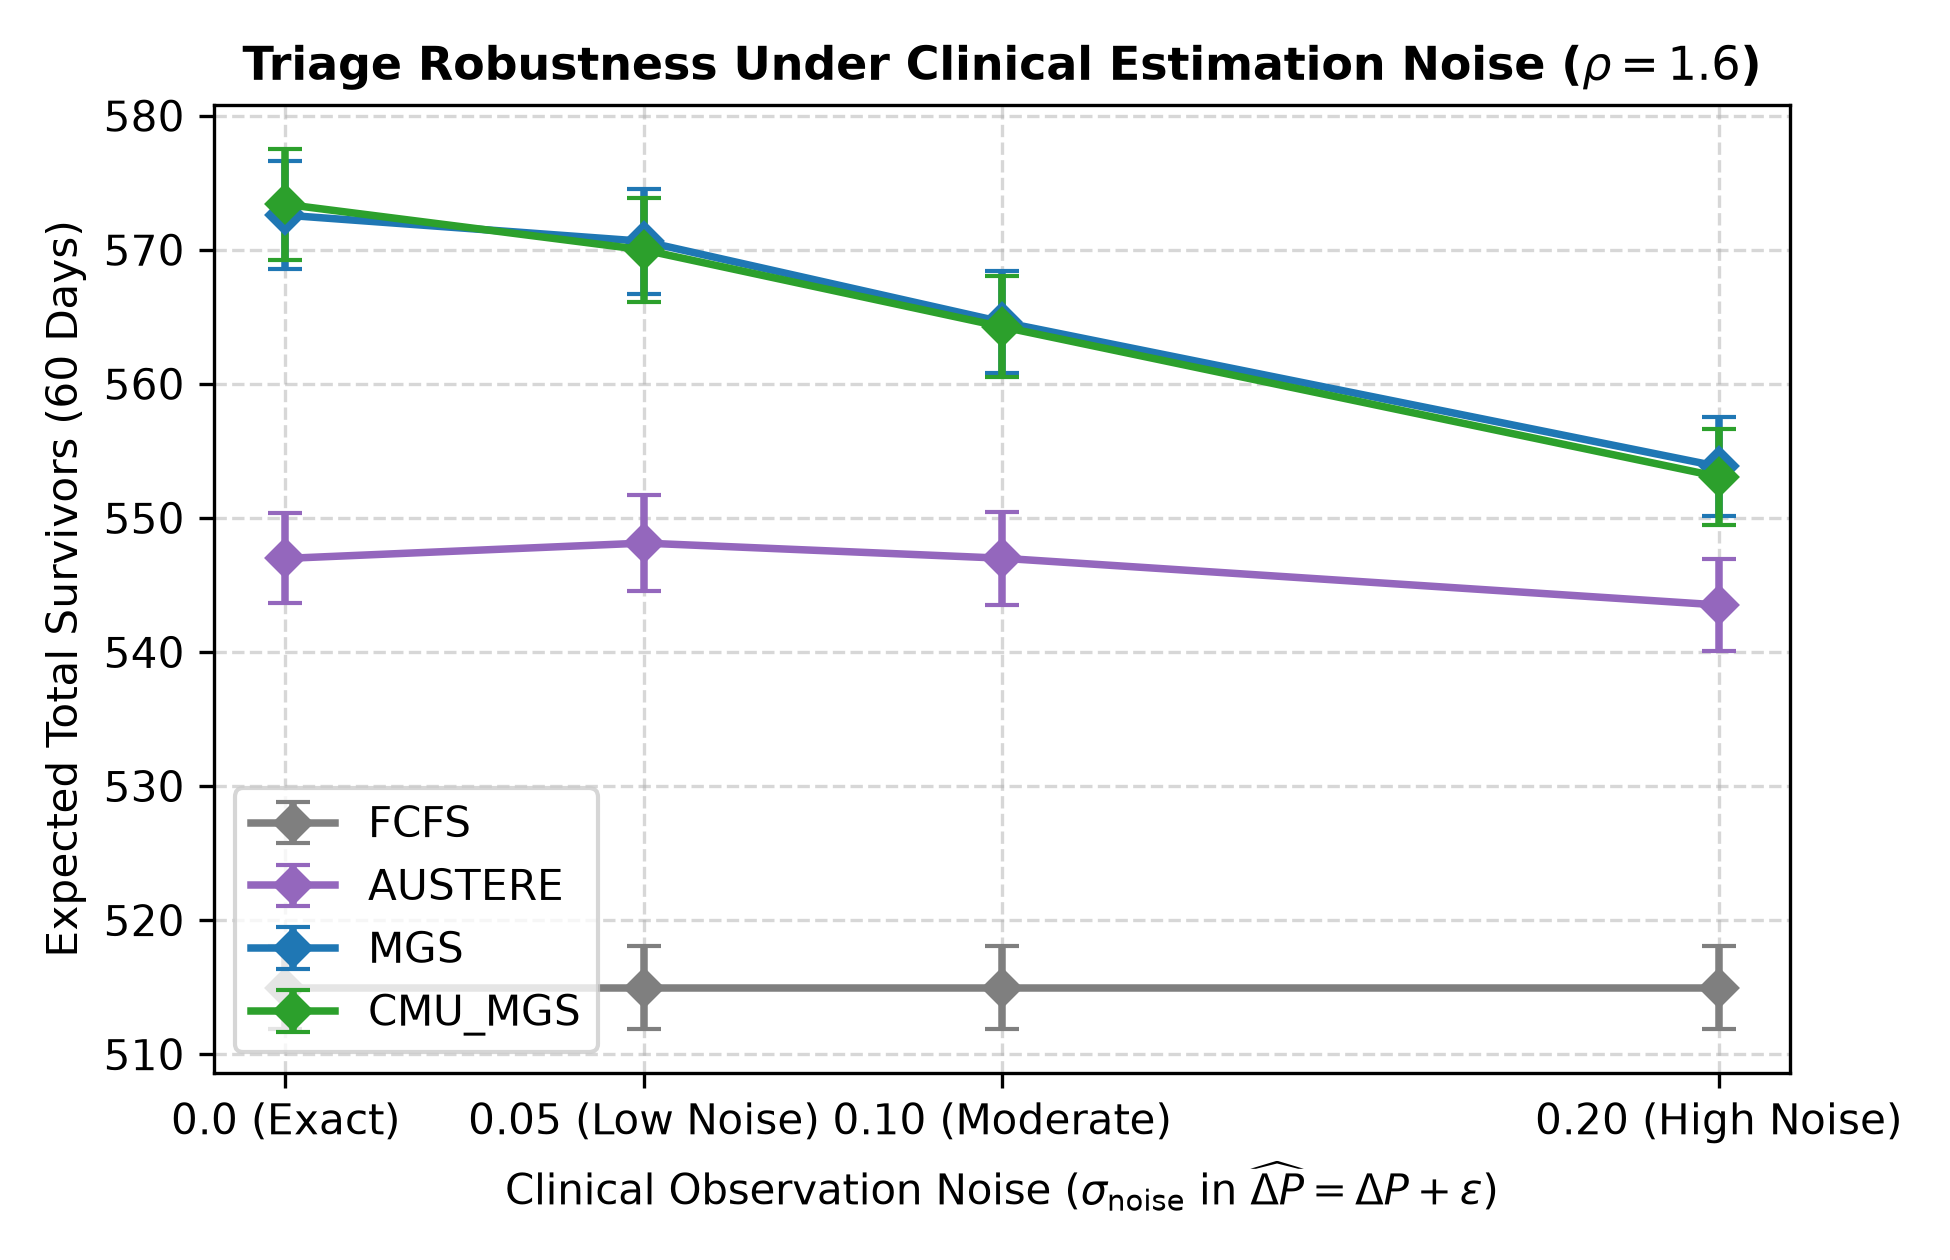
\includegraphics[width=\columnwidth]{fig_sensitivity.png}
\caption{Expected survivors under noisy $\widetilde{\Delta P}$ at $\rho=1.6$. Benefit-based policies remain superior to FCFS for $\sigma\le 0.2$.}
\label{fig:sensitivity}
\end{figure}

\section{Limitations}
\label{sec:limitations}

Only bed capacities are empirically calibrated; $P_{\mathrm{in}}$, $P_{\mathrm{out}}$, $W_{\max}$ and LOS parameters are synthetic and shared across age groups. No nurse staffing, cleaning delays, early discharge, or step-down blocking are modeled. Overflow is restricted to adult--coronary beds. $\Delta P$ is treated as an observable clinical score (possibly noisy), not as an estimated causal effect from observational data. Normative claims are therefore conditional on the modeled objective of maximizing expected survivors under known (or noisy) salvage margins, not a full ethical analysis of equity across demographic groups.

\section{Conclusions}
\label{sec:conclusion}

We presented a DES of multi-type ICU triage with waiting-time deterioration, severity-dependent LOS, adult--coronary overflow and imperfect information. Using HU-UFMA/CNES capacities and synthetic clinical distributions, CRN experiments show that benefit-per-bed-day ranking (CMU-MGS) and marginal-gain ranking (MGS) dominate FCFS, MSF, LSF and a deadline-aware austere heuristic under surge, while remaining robust to moderate noise in $\widetilde{\Delta P}$. At low congestion, statistical differences exist under CRN but are negligible in relative magnitude. Operationally, hospitals facing sustained ICU scarcity should prefer indices that combine salvageability with expected bed holding time, while recognizing that $\Delta P$ estimation error and equity constraints must be governed clinically.

\section*{Data and code availability}
Bed-capacity extracts, experiment configurations, simulation code, raw replication outputs and figure scripts are included in the project repository accompanying this manuscript. CNES bed counts are publicly available from DATASUS \cite{cnes_datasus_huufma}.

\section*{CRediT authorship contribution statement}
\textbf{Carlos Eduardo Veras Gomes:} Software, Investigation, Visualization, Writing -- original draft.
\textbf{Jo\~ao Augusto Ferreira Nunes de Carvalho:} Software, Validation, Data curation.
\textbf{Francisco Glaubos Nunes Cl\'imaco:} Conceptualization, Methodology, Supervision, Writing -- review \& editing.

\section*{Declaration of competing interest}
The authors declare that they have no known competing financial interests or personal relationships that could have appeared to influence the work reported in this paper.

\bibliographystyle{elsarticle-num}
\bibliography{bib}

\end{document}
